\documentclass[a4paper]{article}

\usepackage[table]{xcolor}%this has to be the first!!!!!!
\usepackage{fullpage} % Package to use full page
%\usepackage{parskip} % Package to tweak paragraph skipping
\usepackage{tikz} % Package for drawing
\usetikzlibrary{shapes,arrows,matrix,positioning}
\usepackage{amsmath}
\usepackage{indentfirst}
\usepackage{hyperref}
\usepackage{subcaption}
\usepackage{graphics}
\usepackage{graphicx}
\usepackage{minted}
\usepackage{multicol}
\usepackage{mathrsfs}
%color define
\definecolor{codebg}{RGB}{230,255,253}
\definecolor{function}{RGB}{210,0,26}
\definecolor{para}{RGB}{255,137,137}
\definecolor{output}{RGB}{238,224,201}
\setminted[cpp]{mathescape=true,breaklines,bgcolor=codebg,linenos}

\tikzset{
  block/.style = {rectangle, draw, fill=output, text width=6cm, text centered, rounded corners, minimum height=4em},
  line/.style = {draw, -latex'},
}

%function newcommand
\newcommand{\func}[1]{\textbf{\textcolor{function}{#1}}}
\newcommand{\para}[1]{\textbf{\emph{\textcolor{para}{#1}}}}

%other examples for icon in text
%WARNING: the number is not allowed in newcommand name
\newcommand{\testA}{\tikz \fill[brown] (2pt,2pt) rectangle (8pt,8pt);}
\newcommand{\testB}{\tikz \fill[black] (3pt,3pt) circle (3pt);}

\usepackage{biblatex}
\addbibresource{bibliography.bib}
\title{vof.h documentation}
\author{Haochen(Langford) Huang}
\date{\today}

\makeatletter%title setting
\def\@maketitle{%
  \newpage
  \null
  \vskip 2em%
  \begin{center}%
  \let \footnote \thanks
    {\LARGE \@title \par}%
    \vskip 1.5em%
    {\Large
      \lineskip .5em%
      \begin{tabular}[t]{c}%
        \@author
      \end{tabular}\par}%
    \vskip 1em%
    {\large \@date\par}%
    \vskip 1em%
    {\large version:draft}%
  \end{center}%
  \par
  \vskip 1.5em}
\makeatother

\begin{document}

\maketitle
\section{Introduction}
\textbf{vof.h} aims to solve advection equation
\begin{equation}\label{equ:advec}
    \frac{\partial c_{i}}{\partial t} + \mathbf{u}\cdot\nabla c_{i} = 0
\end{equation}
where $c_{i}$ is the volume fraction.
Additionally, Basilisk provides option to compute transport equation of diffusive tracer which is confined within specific phase e.g. ions in fluids whose governing equation reads\cite{2015_Lopez}
\begin{equation}\label{equ:advectr}
    \frac{\partial t_{i,j}}{\partial t} + \mathbf{u}\cdot\nabla t_{i,j} = 0
\end{equation}
where $t_{i,j}=f_{j} c_{i}$ or $tr=f_{j} (1-c_{i})$ depending on which side the tracer is confined. $f_{j}$ is the concentration of the tracer.\par
The documentation is split into two parts: in the first part, the preparation to sovle the equation including gradient computation, prolongation in tree-grid and default event settings to implement prolongation are introduced. The solution of equation \ref{equ:advec} and \ref{equ:advectr} are carefully discussed in the second part.

\section{Preparation}
\subsection{\func{vof\_concentration\_gradient}}\label{sec:gradient}
\func{vof\_concentration\_gradient} computes gradient for vof concentration using three-point scheme when given position is away from the surface and two-point scheme for those surface nearby cells.
\subsubsection{Parameters}
\begin{table}[h]
  \centering
  \begin{tabular}{|c|c|c|c|c|}
    \hline
    Name & Data type & Status & Option & Representation (before/after)\\[0.5ex]
    \hline\hline
    \rowcolor{output} gradient & double & \textbf{output} & output & $\nabla t_{i,j}$\\
    \hline
    \para{point} & Point & unchanged & complusory & position index\\
    \hline
    \para{c} & scalar & unchanged & complusory & volume fraction $c_{j}$\\
    \hline
    \para{s} & scalar & unchange & complusory & $t_{i,j}$\\
    \hline
  \end{tabular}
\end{table}
\subsubsection{Worth Mentioning Details}
The gradient is calculated following a upwind-type two-point scheme when locates near the surface cell. In particular, such scheme is active if the volume fraction of only one adjacent cell is greater than $0.5$. Otherwise a central three point scheme is used. Notably, the gradient is valid only if there are at least two out of adjacent cells, including current one, has fraction volume greater than $0.5$.
\subsubsection{Program Workflow}
\begin{multicols}{2}
  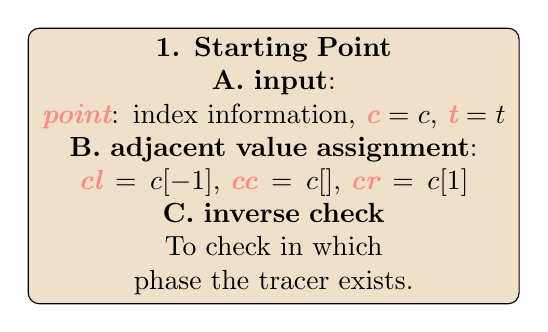
\begin{tikzpicture}
    \node [block]{
        \textbf{1. Starting Point}\\
        \textbf{A. input}:\\
        \para{point}: index information, $\para{c}=c$,  $\para{t}=t$\\
        \textbf{B. adjacent value assignment}:\\
        $\para{cl}=c[-1]$, $\para{cc}=c[]$, $\para{cr}=c[1]$\\
        \textbf{C. inverse check}\\
        To check in which phase the tracer exists.
      };
  \end{tikzpicture}
 \columnbreak
 \begin{minted}{cpp}
foreach_dimension()
static double vof_concentration_gradient_x (Point point, scalar c, scalar t)
{
  static const double cmin = 0.5;
  double cl = c[-1], cc = c[], cr = c[1];
  if (t.inverse)
    cl = 1. - cl, cc = 1. - cc, cr = 1. - cr;
 \end{minted}
\end{multicols}

\begin{center}
  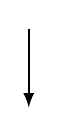
\begin{tikzpicture}
    \draw[-latex,thick](0,0) -- (0,-1); 
  \end{tikzpicture}
\end{center}

\begin{multicols}{2}
  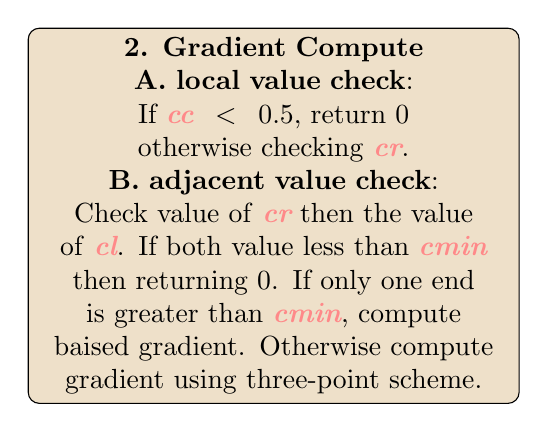
\begin{tikzpicture}
    \node [block]{
        \textbf{2. Gradient Compute}\\
        \textbf{A. local value check}:\\
        If $\para{cc}<0.5$, return $0$ otherwise checking \para{cr}.\\
        \textbf{B. adjacent value check}:\\
        Check value of \para{cr} then the value of \para{cl}. If both value less than \para{cmin} then returning $0$. If only one end is greater than \para{cmin}, compute baised gradient. Otherwise compute gradient using three-point scheme.
      };
  \end{tikzpicture}
 \columnbreak
 \begin{minted}{cpp}
  if (cc >= cmin && t.gradient != zero) {
    if (cr >= cmin) {
      if (cl >= cmin) {
	if (t.gradient)
	  return t.gradient (t[-1]/cl, t[]/cc, t[1]/cr)/Delta;
	else
	  return (t[1]/cr - t[-1]/cl)/(2.*Delta);
      }
      else
	return (t[1]/cr - t[]/cc)/Delta;
    }
    else if (cl >= cmin)
      return (t[]/cc - t[-1]/cl)/Delta;
  }
  return 0.;
}
 \end{minted}
\end{multicols}
\subsection{\func{vof\_concentration\_refine}}
\func{vof\_concentration\_refine} defines the prolongation formula of VOF-concentration $t$ when mesh is refined.
\subsubsection{Parameters}
\begin{table}[h]
  \centering
  \begin{tabular}{|c|c|c|c|c|}
    \hline
    Name & Data type & Status & Option & Representation (before/after)\\[0.5ex]
    \hline\hline
    \para{point} & Point & unchanged & complusory & position index\\
    \hline
    \para{s} & scalar & unchange & complusory & $t_{i,j}$\\
    \hline
  \end{tabular}
\end{table}
\subsubsection{Worth Mentioning Details}
\begin{figure}[!htbp]
    \centering
    \begin{subfigure}[b]{0.45\textwidth}
        \centering
        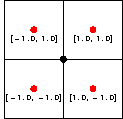
\includegraphics[height=5.5cm]{image/child.pdf}
        \subcaption{}
        \label{fig:child_a}
    \end{subfigure}
    \begin{subfigure}[b]{0.45\textwidth}
        \centering
        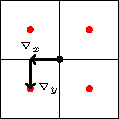
\includegraphics[height=5.5cm]{image/childgradient.pdf}
        \subcaption{}
        \label{fig:child_b}
    \end{subfigure}
    \caption{(a) Sketch for $child$ index. (b) Sketch for volume-fraction-weighted linear interpolation.}
    \label{fig:child}
\end{figure}
Basilisk employs $child$ index to indicate spatial relation between parent and child cells, as displayed in figure \ref{fig:child_a}, the child cells with greater $x$ (resp. $y$) coordinate are assigned with $child.x = 1$ (resp. $child.y = 1$) vice versa. When calling the macro $foreach_child$, Basilisk will automatically transversal every child cells and $child$ index is assigned with corresponding value. As indicated by figure \ref{fig:child_b}, given an active value, the prolongation is achieved by employing linear interpolation all the way to the center of child cell. Take 2D case as an example, the prolongation result $t_{child}$ is obtained by 
\begin{equation}\label{equ:prolongation}
    t_{child} = c_{child}(\frac{t_{parents}}{c_{parents}} + \frac{\Delta}{4}(child.x\nabla_xt+child.y\nabla_yt))
\end{equation}
where $c$ is the fraction volume which is different for parent cell and child owing to reconstruction and $\Delta_xt,\Delta_yt$ are gradient computed by \func{vof\_concentration\_gradient} which has been detailed discussed in previous section.

\subsubsection{Program Workflow}
\begin{multicols}{2}
  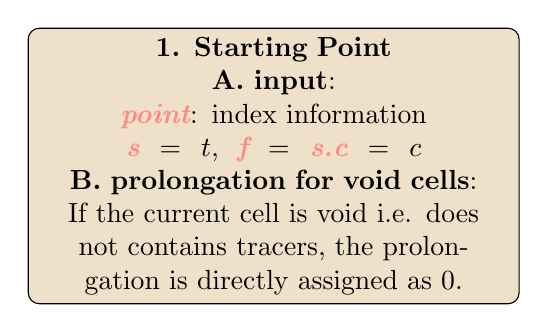
\begin{tikzpicture}
    \node [block]{
        \textbf{1. Starting Point}\\
        \textbf{A. input}:\\
        \para{point}: index information\\ $\para{s}=t$, 
 ~$\para{f}=\para{s.c}=c$\\
        \textbf{B. prolongation for void cells}:\\
        If the current cell is void i.e. does not contains tracers, the prolongation is directly assigned as $0$.\\
      };
  \end{tikzpicture}
 \columnbreak
 \begin{minted}{cpp}
#if TREE
static void vof_concentration_refine (Point point, scalar s)
{
  scalar f = s.c;
  if (cm[] == 0. || (!s.inverse && f[] <= 0.) || (s.inverse && f[] >= 1.))
    foreach_child()
      s[] = 0.;
 \end{minted}
\end{multicols}

\begin{center}
  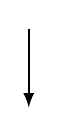
\begin{tikzpicture}
    \draw[-latex,thick](0,0) -- (0,-1); 
  \end{tikzpicture}
\end{center}

\begin{multicols}{2}
  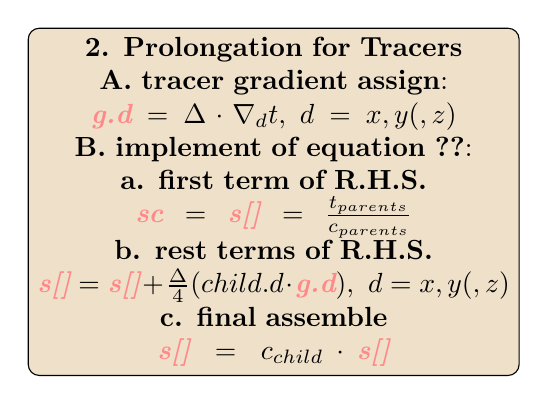
\begin{tikzpicture}
    \node [block]{
        \textbf{2. Prolongation for Tracers}\\
        \textbf{A. tracer gradient assign}:\\
        $\para{g.d}=\Delta\cdot\nabla_dt,\ d = x,y(,z)$\\
        \textbf{B. implement of equation \ref{equ:prolongation}}:\\
        \textbf{a. first term of R.H.S.}\\
        $\para{sc}=\para{s[]}=\frac{t_{parents}}{c_{parents}}$\\
        \textbf{b. rest terms of R.H.S.}\\
        $\para{s[]}=\para{s[]}+\frac{\Delta}{4}(child.d\cdot\para{g.d}),\ d = x,y(,z)$\\
        \textbf{c. final assemble}\\
        $\para{s[]}=c_{child}\cdot \para{s[]}$
      };
  \end{tikzpicture}
 \columnbreak
 \begin{minted}{cpp}
  else {
    coord g;
    foreach_dimension()
      g.x = Delta*vof_concentration_gradient_x (point, f, s);
    double sc = s.inverse ? s[]/(1. - f[]) : s[]/f[], cmc = 4.*cm[];
    foreach_child() {
      s[] = sc;
      foreach_dimension()
	s[] += child.x*g.x*cm[-child.x]/cmc;
      s[] *= s.inverse ? 1. - f[] : f[];
    }
  }
}
 \end{minted}
\end{multicols}

\section{Advection Solution}
The exact solution is introduced in this section. Before diving into details, the conception of VOF method and major problem confronted in this method shall be discussed first.
\subsection{VOF method}
Generally speaking, there are two steps to accomplish VOF method i.e. advection of volume fraction and reconstruction of surface. The latter one is tackled in headfile \textbf{geometry.h} and will not be covered in this document.\par
 The integral form of equation \ref{equ:advec} is
\begin{equation}
    \Delta^{d} c_i|^{n+1}_{n} + \int_{\Omega}\mathbf{u}_f\cdot\nabla c_i= 0
\end{equation}
where $\Delta^d$ stands for the area (volume) of the cell.
Using divergence theorem the equation turns into
\begin{equation}\label{equ:advec2}
    \Delta^{d} c_i|^{n+1}_{n} + \int_{\partial\Omega}\mathbf{u}_f c_i - \int_{\Omega}c_i\nabla\cdot \mathbf{u}_f= 0
\end{equation}
the second term in equation \ref{equ:advec2} is the face flux $\mathbf{u}_fc_i=\mathbf{F}$. Consider the conservative constraint $\nabla\cdot\mathbf{u}=0$, the third term is supposed to vanish. However, as will be discussed later, such term plays a critical role in the overall algorithm.\par
The advection is achieved by applying operator-split advection method\cite{2011_Gretar} wherein the volume fraction is transport in each dimension. Take 2D case as an example, equation \ref{equ:advec2} now reads
\begin{align}
    c_i^\ast = c_i^{n} - \frac{\Delta t}{\Delta}(\mathbf{F}_x[1]-\mathbf{F}_x[]) + \frac{\Delta t}{\Delta}\int_{\Omega}c_i\nabla_x\cdot\mathbf{u}_f\label{equ:advec3x}\\
    c_i^{n+1} = c_i^\ast - \frac{\Delta t}{\Delta}(\mathbf{F}_y[1]-\mathbf{F}_y[]) + \frac{\Delta t}{\Delta} \int_{\Omega}c_i\nabla_y\cdot\mathbf{u}_f
\end{align}
Given interface and non-divergence face velocity $\mathbf{u}_f$ at $t^n$ assuming the time step between $t^{n}$ and $t^{n+1}$ is $\Delta t$, the very next step is to obtain the face flux $\mathbf{F}$. The sketch of advection for specific cell is demonstrated by figure \ref{fig:VOFadvection}. The gray area represents volume of fraction and corresponding interface.
The face flux $\mathbf{F}$ is directly obtained by the gray area within dashed rectangle whose width is $\mathbf{u}_f\Delta t$. To avoid non-conservation induced by transporting overlapped area (the blue area in figure \ref{fig:VOFadvectiony}), reconstruction is applied between advection of every direction as indicated from shape changes between two figures.\par
Yet there is still one constraint to satisfy: the volume fraction should be $0\leq c_i \leq1$ at any stage. However without additional care, such rule can be violated between direction switch. Take condition in figure \ref{fig:VOFadvectionx} as an example. Assume $c^n=0.9,u_f.x[]=0.3,u_f.x[1]=0.1$, for sake of simplicity the time step and cell width are set to be unity. Ignoring the third term in equation \ref{equ:advec3x}, $c^\ast = 1.1 > 1.0$ which of course break the constraint and leads to failure in surface reconstruction. An opposite condition may also occur where the volume fraction eventually becomes $c<0$.
The dilation term (third term in equation \ref{equ:advec2}) is therefore introduced to cope with such issue\cite{2003_Scardovelli}.\par
\begin{figure}[!htbp]
    \centering
    \begin{subfigure}[b]{0.45\textwidth}
        \centering
        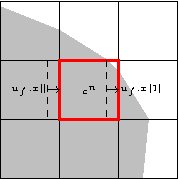
\includegraphics[height=5.5cm]{image/VOFadvectionx.pdf}
        \subcaption{}
        \label{fig:VOFadvectionx}
    \end{subfigure}
    \begin{subfigure}[b]{0.45\textwidth}
        \centering
        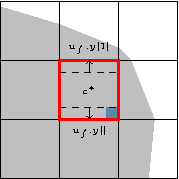
\includegraphics[height=5.5cm]{image/VOFadvectiony.pdf}
        \subcaption{}
        \label{fig:VOFadvectiony}
    \end{subfigure}
    \caption{Sketches for (a) advection on x direction (b) advection on y direction. The width of dashed rectangle is $\mathbf{u}_f\Delta t$}
    \label{fig:VOFadvection}
\end{figure}

\subsubsection{The dilation term}
Given the non-divergence of $\mathbf{u}_f$, the dilation term in equation \ref{equ:advec2} can be rewrite in discrete form as:
\begin{equation}\label{equ:dilation}
    \int_{\Omega}c_i\nabla\cdot\mathbf{u}_f = g\Delta^{d-1} \sum_d(u_f.d[1]-u_f.d[])
\end{equation}
where $g$ is an arbitrary value and can even vary in different cells or in different cycle of iteration. The main topic in this section is to find a proper form of $g$ which can help to overcome the overfull issue depicted previously.\par
The condition where $g=0$ i.e. no dilation has been fully discussed, consider now the condition where $g=1$. Take condition in figure \ref{fig:dilation1} as an example. The volume fraction for current cell is $c^n = 1$, given the input face velocity on both faces, the overfull occurs without dilation term. However after adding the dilation, according to equation \ref{equ:advec3x} and \ref{equ:dilation} the input flux $\mathbf{F}$ (gray area confined by dashed rectangle) will be counteracted by dilation term (area of dashed rectangle when $g=1$). The difference between (blue area) prevents the overfull issue.\par
\begin{figure}[!htbp]
    \centering
    \begin{subfigure}[b]{0.45\textwidth}
        \centering
        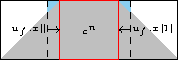
\includegraphics[height=1.83cm]{image/dilation1.pdf}
        \subcaption{}
        \label{fig:dilation1}
    \end{subfigure}
    \begin{subfigure}[b]{0.45\textwidth}
        \centering
        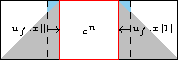
\includegraphics[height=1.83cm]{image/dilation2.pdf}
        \subcaption{}
        \label{fig:dilation2}
    \end{subfigure}
    \caption{Sketch for dilation. The area highlighted by blue represents the area difference induced by adding dilation term}
    \label{fig:dilation}
\end{figure}
Nevertheless, the dilation can be harmful at certain circumstance. As shown by figure \ref{fig:dilation2} where the volume fraction now becomes $c^n=0$, with input face velocity the dilation now promotes clipping ($c<0$) owing to area difference (blue area).
\subsubsection{Coefficient $g$ and CFL number}
Basilisk follows work by Weymouth and Yue\cite{2010_Weymouth} and sets coefficient $g$ as 
\begin{equation}\label{equ:gcorrect}
    g=c_c=\left\{
    \begin{array}{cc}
    1     &  c^n \geq 0.5\\
    0     &  c^n <0.5
    \end{array}
    \right.
\end{equation}
with CFL number constraint $\sum_d \frac{\Delta t}{\Delta}|u_f.d|<0.5$ the method can preserve exact conservation.\par
Following the same work, given $g$ in equation \ref{equ:gcorrect} the restriction for volume fraction reads
\begin{align}
    c\geq0.5\geq min(\frac{\Delta t}{\Delta} u_f[1],f)+\frac{\Delta t}{\Delta}(u_f[]-u_f[1]);&\  1-c\geq0.5\geq \frac{\Delta t}{\Delta}u_f[]-max(0,\frac{\Delta t}{\Delta}u_f[1]-1+c)\\
    c\geq0.5\geq \frac{\Delta t}{\Delta}(u_f[]-u_f[1]);&\  1-c\geq0.5\geq \frac{\Delta t}{\Delta}(u_f[]-u_f[1])\label{equ:restriction}
\end{align}
with CFL$<0.5$, the restriction can be easily satisfied therefore preserving the volume conservation. Note however such restriction is deduced based on the assumption that the volume fraction of current cell is the only accessible.

\subsection{\func{sweep\_x}}
\func{sweep\_x} aims to achieve advection equation \ref{equ:advec3x} in each direction. Notably, similar method is also applied to the advection of tracer in which the dilation term is added.
\subsubsection{Parameters}
\begin{table}[h]
  \centering
  \begin{tabular}{|c|c|c|c|c|}
    \hline
    Name & Data type & Status & Option & Representation (before/after)\\[0.5ex]
    \hline\hline
    \rowcolor{output} \para{c} & scalar & \textbf{updated} & compulsory & $c^n$/$c^\ast$\\
    \hline
    \para{cc} & scalar & unchanged & complusory & $c_c$ in equation \ref{equ:gcorrect}\\
    \hline
    \para{tcl} & scalar & unchanged & complusory & tracer coefficient $t_c$\\
    \hline
  \end{tabular}
\end{table}
\subsubsection{Worth Mentioning Details}
The dilation coefficient for tracer advection is defined as 
\begin{equation}
    t_c=\left\{
    \begin{array}{cc}
        t_{ij}/c_i & c^n\geq0.5 \\
        t_{ij}/c_i & c^n<0.5
    \end{array}
    \right.
\end{equation}
Note if inverse is true, the $c_i$ changes as $(1-c_i)$. Different from volume fraction advection, the face flux for tracer is computed using 1D BCG scheme.
\begin{equation}
    \mathbf{F}_t[] = u_f[]\cdot c^\ast[](\frac{t[]}{c^n[]}+\frac{\Delta}{2}[s_d-\frac{\Delta t}{\Delta}u_f[]]\frac{\partial t[]}{\partial x})
\end{equation}
Where the gradient is compute by interface biased scheme introduced in section \ref{sec:gradient} and $s_d$ is the upwind coefficient (see 'bcg.h documentation' for more).
Owing to change of volume fraction, the current volume fraction should be updated by multiplying the latest volume fraction $c^\ast$. The advection for tracer now yields
\begin{equation}
    t^\ast_d = t^n - \frac{\Delta t}{\Delta}(\mathbf{F}_{t,d}[1]-\mathbf{F}_{t,d}[]) + \frac{t_c\Delta t}{\Delta}(u_{f,d}[1]-u_{f,d}[])
\end{equation}
The function is replicated into \func{sweep\_y} and \func{sweep\_z} by macro $foreach\_dimension()$.
\subsection{\func{vof\_advection}}
The VOF advection along with tracer advection is assembled in function \func{vof\_advection}.
\subsubsection{Parameters}
\begin{table}[h]
  \centering
  \begin{tabular}{|c|c|c|c|c|}
    \hline
    Name & Data type & Status & Option & Representation (before/after)\\[0.5ex]
    \hline\hline
    \rowcolor{output} \para{interfaces} & scalar* & \textbf{updated} & compulsory & $c_i^n$/$c_i^{n+1}$\\
    \hline
    \para{i} & int & unchanged & complusory & number of time step\\
    \hline
  \end{tabular}
\end{table}
\subsubsection{Worth Mentioning Details}
Direction switch is implemented by counting the time step $i$. 
\begin{equation}
    D = (i+d)\ mod \ 3 \quad d = 0,1,2\cdots
\end{equation}
Where $D = 0,1,2$ indicates $x,y,z$ direction and shows up in specific sequence depending on $i$.
\section{Draft}
If all the volume fraction is known, flux $\mathbf{F}$ on each face is
\begin{align}
    min(u_f[],c[-1])\geq F[] \geq max(0,u_f[]-\bar{c}[-1])\quad &u_f[]\geq0\\
    -max(0,-u_f[]-\bar{c}[])\geq F[] \geq -min(-u_f[],c[])\quad &u_f[]<0
\end{align}
The flux difference $\Delta F_d[] = F_d[]-F_d[1]$ therefore is
\begin{align}
    min(u_f[],c[-1])-max(0,u_f[1]-\bar{c}[])\geq \Delta F[]\geq max(0,u_f[]-\bar{c}[-1]) - min(u_f[1],c[])\quad &u_f[]>0,u_f[1]>0\\
    min(u_f[],c[-1]) + min(-u_f[1],c[1])\geq \Delta F[]\geq max(0,u_f[]-\bar{c}[-1]) + max(0,-u_f[1]-\bar{c}[1])\quad &u_f[]>0,u_f[1]<0\\
    -max(0,-u_f[]-\bar{c}[])-max(0,u_f[1]-\bar{c}[])\geq \Delta F[]\geq -min(-u_f[],c[]) - min(u_f[1],c[])\quad &u_f[]<0,u_f[1]>0\\
    -max(0,-u_f[]-\bar{c}[])+ min(-u_f[1],c[1])\geq \Delta F[]\geq -min(-u_f[],c[]) + max(0,-u_f[1]-\bar{c}[1])\quad &u_f[]<0,u_f[1]<0
\end{align}
\printbibliography
\end{document}
